\documentclass[preprint]{iucr}
 \journalcode{J}
 \papertype{CP}

\usepackage{graphicx}
\usepackage{minted}

\usepackage[T1]{fontenc}
\usepackage[utf8]{inputenc}

\begin{document}

\title{The Fast Azimuthal Integration Python library}
\shorttitle{PyFAI}

    \author[a]{Aurore}{Deschildre}
    \author[a]{Giannis}{Ashiotis}
    \author[b]{Zubair}{Nawaz}
    \author[a]{Jonathan P.}{Wright}
    \author[a]{Dimitrios}{Karkoulis}
    \author[c]{Fr\'ed\'eric-Emmanuel}{Picca}
    \cauthor[a]{J\'er\^ome}{Kieffer}{jerome.kieffer@esrf,fr}{}
    \aff[a]{European Synchrotron Radiation Facility, \city{Grenoble}, \country{France}}
    \shortauthor{Kieffer et al.}

\maketitle

\begin{synopsis}
The Python library for high performance azimuthal integration 
\end{synopsis}

\begin{abstract}
PyFAI is an opensource software package designed to perform azimuthal and radial integration and,
correspondingly, 2D regrouping on area detector frames for SAXS, WAXS and XRPD
experiments. It is written in Python, a language widely accepted and used by the scientific community today, which enables
the users to easily incorporate the PyFAI libraries into their processing pipeline. We present recent work
which focuses both on the accuracy of the results and execution speed.
\end{abstract}

\section{Introduction}
Azimuthal integration allows using area detectors for recording powder
diffraction patterns, which  ensure larger solid angle coverage and hence a better harvest of X­ray photons. 
This data reduction 
step is one of the most time ­consuming tasks in the processing pipeline and
sometimes limits the productivity of modern synchrotron beamlines, where
diffraction is used to probe samples with a  pencil beam in 2D raster scans or
diffraction tomography experiments by using very fast detectors. 

This contribution describes the Python library pyFAI in its version 0.9.5 (fall
2014) which can be used to calibrate the experimental setup of a powder
diffraction experiment or a SAXS experiement using area detector using
Debye-Scherrer rings of a reference compound. 
Afer describing how the geometry is internally represented, the various
image analysis algorithm used to extract Debye-Scherrer rings are presented.
Those ring positions are combined with a calibrant to perform the refinement
of the geometry.

Once this geometry known, azimuthal regrouping can be performed. 
PyFAI implements various algorithm for intergrating with various pixel splitting
schemes which will be exposed. 
The latest algorithms have been optimized for
manycore computer devices.
%, they are benchamarked with previous implementation
%on many classes of devices.

Finally some scientific examples are given on how pyFAI can be used to decompose 
diffraction images into amorphous and Bragg component and its application
to serial crystallography.
 
\section{Experiment description}
In pyFAI, a basic experiment is defined by an area-detector which position in
space is defined versus the intersection of the incoming pencil beam and the
sample plan.

\subsection{Detector}
Like most other image processing packages, pyFAI allows the definition of 2D
detectors by a constant pixel size (in meter) but this approach shows its limits
with various types of detectors.
Large area pixel detector are often composed from the assembly of smaller
modules (Pilatus from Dectris, Maxipix from ESRF, \ldots). 
By construction, such detector exhibit gaps between modules and pixels of
various sizes within a module, hench requires a specific mask.
Optically coupled CCD detector should also be corrected
for small spacial displacement of the pixel, often called geometric distortion.

\subsubsection{Detectors classes} are used to define a familly of detectors/ 
To take the specificites of each detector into account, pyFAI contains about
40 detectors class definition which contains the mask (invalid pixels, gaps,
\ldots) and a method to calculate the pixel position in cartesian coordinates.
For tapper coupled CCD detectors, the geometrical distortion is often
described as a bi-dimentional cubic spline and save in a so called ``spline
file''. 
Such files have been introduced by FIT2D \cite{fit2d} and are still widely
used. PyFAI can create a detector description by loading into a ``FReLon''
detector object

\subsubsection{Nexus Detectors}
Any detector object in PyFAI, can be saved to a HDF5 file following the NeXus
conversion (slightly modified).
Detector objects can then be restored from the disk, making detector definition
less error-prone.
Pixels of a 2D detector are saved as a 4D HDF5-dataset: 2D array of vertices
pointing to every corner of each pixel, which makes an array of shape: (ny, nx, 4, 3)
This can define detectors no longer planar, like tiled detectors from
ImXpad or the Pilatus12M from Dectris, even accounting for the normal of each
pixel. 
While extremely flexible, this detector definition come at the cost of
large description files.

\subsection{Geometry}
The experiment geometry is defined in pyFAI by six parameters: the sample
detector distance along with the detector coordinates of the sample's orthogonal
projection on the detector plane, called PONI. 
The detector's rotation along the three axes are completing those six
parameters. 
All three distances are given in meter and all three rotation are given
in radians.
Those S.I. units may look inaddapted or odd to users familiar to other code
like FIT2D \cite{fit2d} or SPD \cite{spd}, therefore the geometry can be
exported to (or imported from) other software.

 
\subsubsection{Binning}
One of the strength of this geometry is capability to perform binning of the
detector without having to re-calibrate or re-calculate the position in space.
All pyFAI detector classes have a binning option which will increase the pixel
size accordingly and divide detector shape accordingly. 
This even works for detectors with distortion files. 

\section{Calibration}
Calibration of the position of the detector is performed using Debye-Scherrer
rings collected from a reference powder called ``calibrant''.
Rings are extracted and control points are located as maxima of those rings.
The geometry of the experiment is obtained from a least-squares refinement of
the $2\theta$ angles.
In this contribution we will call them ``ring'' even if, for planar detector,
they are actually conics formed by the intersection of the Debye-Scerrer cones
with the detector plan. 
PyFAI does not assume rings are circles, ellipses or parabola and is able to fit
any kind of geometry. The support for the geometry refinement of non planar
detector is still under development.

\subsection{Calibrant}
PyFAI provides ten calibrants files among the most used ones: ceria, corundum,
gold, lantahnide hexaboride and silicon for powder diffraction; silver behenate,
tetradecanol and para-bromobenzoic acid for small angle scattering.
Any file containing d-spacing in angstrom can be used as calibrant for a
geometry calibration and can be loaded by the $Calibrant$ class instance.
This computer object is in charge of
calculating the reference $2\theta$ cone opening 
against which the geometry will be refined (provided the wavelength/energy is
known).

\subsection{Peak-picking}
With the nano-focused beam available on modern synchrotron facilities
\cite{id13}, fewer crystal get hit by the beam going through the
sample making Debye-Scherrer ring obtained from the diffraction of reference
powders spotty.
As grinding reference powder is not advices (it would at least broaden peaks if
not changing crystal structure), we decided to address this issue by image analysis 
and reconstruct Debye-Scherrer rings.
An alternative approach is to use single crystal indexation technics, for
example using the Fable software \cite{bonnin}.

\subsubsection{Massif extraction}
\label{massif}
allows a clear separation between regions containing large
photon counts (rings) and the background.
It uses a difference of the image with itself, blured with a given width,
$\sigma$. 
Border of the regions with high intensity are negative in this
difference with a gaussian image, so positive region are labeled and represents
a ring (or a fraction of it). Peaks, which are local maxima, are sample within
the same region.
The width of the gaussian has to be larger than the typical distance
between two peaks within a ring and smaller than the distance between two
rings. 
PyFAI includes some heuristics to guess an acceptable parameter in most cases
but they can be overridden by the command line argument $--gaussian=XX$.

\subsubsection{Sub-pixel precision} 
\label{subpixel}
on the peak position is obtained using a second order developemnt of the
intensity on the vinicy of the peak:
$$ I(\overrightarrow{x}) = I(\overrightarrow{x_0}) + \nabla
I(\overrightarrow{x_0})\cdot (\overrightarrow{x}-\overrightarrow{x_0}) +
\frac{1}{2} (\overrightarrow{x}-\overrightarrow{x_0})^T\cdot\mathcal{H}
I(\overrightarrow{x_0})\cdot(\overrightarrow{x}-\overrightarrow{x_0})$$ which
can be derived into:
$$\nabla I(\overrightarrow{x}) =\nabla I(\overrightarrow{x_0}) +
\mathcal{H}I(\overrightarrow{x_0})\cdot(\overrightarrow{x}-\overrightarrow{x_0})$$
Extrema are define by $\nabla I(\overrightarrow{x})=0$, hence:
$$\overrightarrow{x} = \overrightarrow{x_0} - (\mathcal{H}
I(\overrightarrow{x_0}))^{-1}\cdot\nabla I(\overrightarrow{x_0})$$ where $I$,
$\nabla I$ and $\mathcal{H} I$ are the scalar field of intensity, its gradient
(vector) and hessian (matrix), respectively, measured at the maximum pixel position.

\subsubsection{Blob detection}
\label{blob}
is a computer vision method which allows to perform peak-picking without
\textit{a-priori} knowledge on the level of the image.
This feature is essential to us as diffraction images exhibit a very large
dynamic range.

The diffraction image is sequencially blured with gaussian filter which
width $\sigma$ follows the geomtric serie: $\frac{1}{2}$,
$\frac{\sqrt{2}}{2}$, 1, $\sqrt{2}$, 2, $2\sqrt{2}$, \ldots
For each blured image at scale $\sigma$, the subsequent blured (at
$\sigma'=\sigma\cdot\sqrt(2)$
is subtracted to create a difference of Gaussian
image (called DoG) which highligths the features of the image which typical size
is $\sigma$. 
A 3D scale-space ($x,y,\sigma$) representation is created from those DoG images.

This method provides us not only the peaks location, as local maxima in
scale-space, but also the typical size of the peak. 
Peak position, scales and intensity are refined as described in the former
paragraph, extended to the scale space.

To keep the computation time reasonable, the implementation of the blob
detection relies on gaussian convolution in real space (i.e. without Fourier
transform), separated in horizontal and vertical direction, with small
convolution kernel of width $8 \sigma +1$.
To prevent the growth of the window with larger $\sigma$, a pyramid of Gaussians
is built by binning the blured image by a factor 2 when it reaches a $\sigma=2$.

The drawback of this algoritm, beside the calcualtion time, is its very high
sensitivity to noise in flat regions. 
This is why blob detection is only used in the re-calibration procedure to
extract all peaks in a region of interest, ROI determined form an
approximative geometry.
Moreover blob detection cannot find peaks wich width is smaller than  
$\sigma=0.7$ which correspond to 3 pixels.

\subsection{User interface}
The calibration tool of pyFAI has been available along with the
integration tool since the very begining of the project as a core idea is to
use the same code to calculate the geometry and to perform the integration,
avoiding any error of copy-paste of coordinates.

The user interface for calibration has improved a lot recently: the assignement
of the ring number is now possible graphically, as shown in figure \ref{calib}.
An rough estimate of the geometry is usually obtained from a mouse click on the
two inner-most rings. 
The blue and green dots correspond to the control points extracted using the
algorithm described in \ref{massif}. 
After refinement of the geometry, six thin, plain curves are drawn on the
image to mark where Debye-Scherrer rings are expected, allowing a visual
validation of the calibration.

\begin{figure}
\label{calib}
\begin{center}
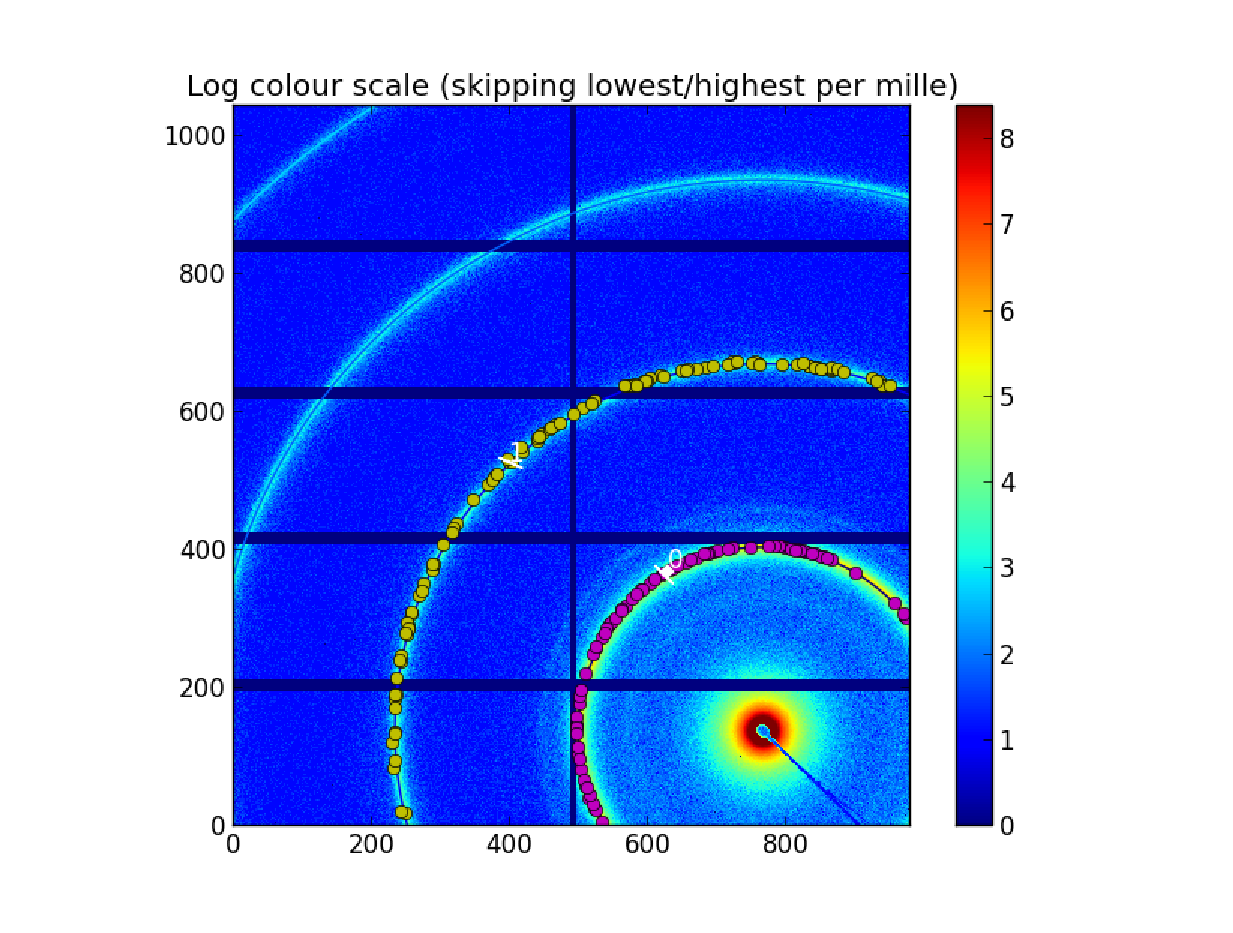
\includegraphics[width=5cm]{calib.eps}
\caption{The calibration window allows manual peak-picking and
ring assignment. A Silver Behenate sample is used as a calibant for the SAXS
beamline BM26/Dubble working at $\lambda=1.0${\AA}}
\end{center}
\end{figure}

From an inital rough calibration, pyFAI allows to perform many operation to
refine all parameters: distance, PONI position, rotation of the detector and
optionnaly the wavelength. The available commands are:
\begin{itemize}
\item help: show the help message
\item abort: quit the program
\item done: performs the azimuthal integration and quits
\item get: prints out the value of a parameter \textem{get wavelength}
\item set: defines the value of a parameter, \textem{set wavelength 1.54e-10} 
\item bound: select the region of validity for a parameter, \textem{ bound dist
0.1 0.5}
\item bounds: review and modify all region of validity for all parameters
\item fix: prevent the parameter to be refined \textem{fix wavelength}
\item free: allows the paramter to be refined \textem{free rot1}
\item refine: re-runs the least squares refinement
\item validate: Estimate the precision of the calibration on the whole
image by overlaying the raw image with the integrated pattern retro-projected.
\item recalib: extract a new set of control points from the n inner most rings
\textem{recalib 5}
\item reset: reset the geometry to its default values,
\item show: prints out the current calibration parameters
\item integrate: performs the 1D and 2D integration to validate the quality of
the calibration.
\end{itemize}

\subsection{Automatic distance/center calibration}
The previous procedure has been automated for specific types of beamlines: 
Macromolecular Crystallography beamlines at the ESRF (MX) need to input the
sample distance togeather with the beam center automatically in the header of
their collected images to be able to process them automatically.
As the area detector is on a moving stage, dictance and center position are
changing from data-collection to data-collection.
The ``MX-calibrate'' tool from pyFAI allows the automatic callibration of
a set of images taken at various distances using Debye-Scherrer rings of a
reference compound (ceria).
After perfroming subsequently peak-picking based on blob-detection and least
square refinement of the geometry on every input frame, distances and
beam-center position are returned as function of the motor position without
human intervention.

\subsection{Graphical user interface}
PyFAI is primarly a Python library, a graphical user interface (GUI) offering
calibration and integration would limit the flexibility of the tool and
constrain the processing piepline. 
Neverthless the Dioptas project 
\cite{diopas}, which is devleopped independently at the APS synchotron, is based
on pyFAI and is offering a graphical user interface for the calibration and
azimuthal integration.

\section{Azimuthal Integration}

The core of pyFAI is to be able to perform azimuthal integration in 1D or 2D as
fast as possible, using python binary extention, often multi-threaded or even
graphics processors (GPU) and other accelerators, while offering a common
interface. 
The implementation details have been described in
\cite{kieffer_ashiotis-proc-euroscipy-2014}.

%\begin{verbatim}
\begin{minted}{python}
import pyFAI, fabio, pylab
ai = pyFAI.load("geometry.poni)
img = fabio.open("imagefile.tif").data
tth, I = ai.integrate1d(img, 1000, method="splitpixel", unit="2th_deg")
pylab.plot(tth, I)
pylab.show()
\end{minted}
%\end{verbatim}
In this sniplet of code one can adapt the number of output points, 
the radial unit ($2\theta$ angle, radius or scattering verctor norm $q$) and the
integration scheme which is summarized into table \ref{methods}.
This table contains 3 pixel splitting schemes: no splitting, splitting of the
bounding box or tight pixel spliting. Each algorithm can be implemented as a
direct transformation like in histogram or using a look-up table.
In this table we summarized in addition the speed-up observed (versus the pure
NumPy \cite{numpy} implementation, on  quad-core computer) and the memory
footprint for integrating a 2048x2048 pixel image into 1000 bins.

\begin{table}[ht]
\caption{Various ``method`` available within pyFAI for azimuthal integration
featuring their speed-up (vs numpy histogram, on a quad-core computer) and
memory footprint for a 2048x2048 pixel image.}
\begin{tabular}[pos]{|c|l|l|l|}
\hline
Pixel split& No splitting & Bounding box & Tight pixel \\
\hline
Direct    & numpy (1x, 324MB) & splitbbox (7x, 327MB) & splitpixel(2x, 479MB)\\
histogram & cython(3x, 323MB) &                       &                \\
\hline
Look-up   & -      & splitBBoxLUT (37x, 672MB)&splitpixelLUT (17x, ?MB)\\
table     &        & splitBBoxCSR (42x, 294MB)&splitpixelCSR (17x, ?MB)\\
\hline
\end{tabular}
\label{table:methods}
\end{table}

It is worth mentioning that while pixel splitting provides smoother results, any
pixel splitting scheme introduces some cross-correlation between neighboring
bins, introducing an overestimation of errors, as described in \cite{billinge2014}.

\section{Signal separation}



\subsection{Diffraction image generation}

Once the geometry defined, the $2\theta$ and $\chi$ position of every single
pixel of the detector are known.
If one assumes the isotropy of signal (real powder without prefered
orientation), $2D$ diffraction patterns can be generated.
The method, $calcfrom1d$ is available from any $Azimuthal Integrator$ or
$Geometry$ instance, is used together with a calibrant object
to generate a fake diffraction image suitable for testing pyFAI or other 
calibration codes (for example to validate the geometry translation from one
program to another).

%\begin{verbatim}
\begin{minted}{python}

import pyFAI, pyFAI.calibrant
det = pyFAI.detectors.detector_factory("pilatus1m")
ai = pyFAI.AzimuthalIntegrator(dist=0.1, poni1=0.1, poni2=0.1, detector=det)
lab6 = pyFAI.calibrant.ALL_CALIBRANTS["LaB6"]
lab6.set_wavelength(1e-10)
img = lab6.fake_calibration_image(ai)
\end{minted}
%\end{verbatim}

In this sniplet of code, after importing the library, a detector is instancated
from its name (line 2) and positionned in space (line 3).
A reference sample is defined on line 4 from the known calibrants and the
wavelength is set on line 5. Line 6 generates a 2D numpy array containing
Debye-Scherrer diffraction ring which can be saved or displayed on the screen.

\subsection{Image offset and validation of the calibration}
By regenerating a 2D diffraction image from the integrated powder pattern one
can assess the quality of the calibration used for the integration.
The calibration tool, pyFAI-calib, offers  a ``validate'' command which measures
the offset on the image (x, y) between the 2D diffraction image and the one
regenerated from the integrated patern, using a phase correlation algorithm.
This allows a measurement of the precision of the PONI, which is often better
than a tenth of a pixel !
To obtain such a result, a proper calibration image with continuous rings (i.e.
not spotty) and a mask to remove the beam stop are mandatory.

\subsection{Amorphous background removal}

PyFAI's azimuthal integrator features a $separate$ method able to separate
the backgound with an azimuthal symmetry (amorphous scattering or powder ring),
from Bragg peaks automatically.

Based on what was described in \cite{PyFAI_PDJ}, a bidimentional azimuthal
integration is performed on the input image.
The output 2D image is filtered out along the azimuthal $\chi$ axis using a
percentile filter to construct the powder diffraction curve without the punctual
Bragg spots.
The number of points in azimuthal and radial direction as well as
the percentile value can be adjusted but the default values are reasonnably
good.

The reconstructed 2D image corresponds to the amorphous/powder/isotropic
composant of the input image and the subtraction of this generated image from
the raw data contains only the bragg signal.
Figure \ref{separate} (left)
presents a close-up look at the first image of a Lysozyme dataset provided by Dectris to
advertize their Pilatus 6M detectors (image taken at the Swiss Light Source). A
moderate ice-ring is clearly visible. After using the automatic amorphous
background removal, which takes into account the mask needed for such pixel
detector, only Bragg peaks remains (right of the image).

\begin{figure}
\label{separate}
\begin{center}
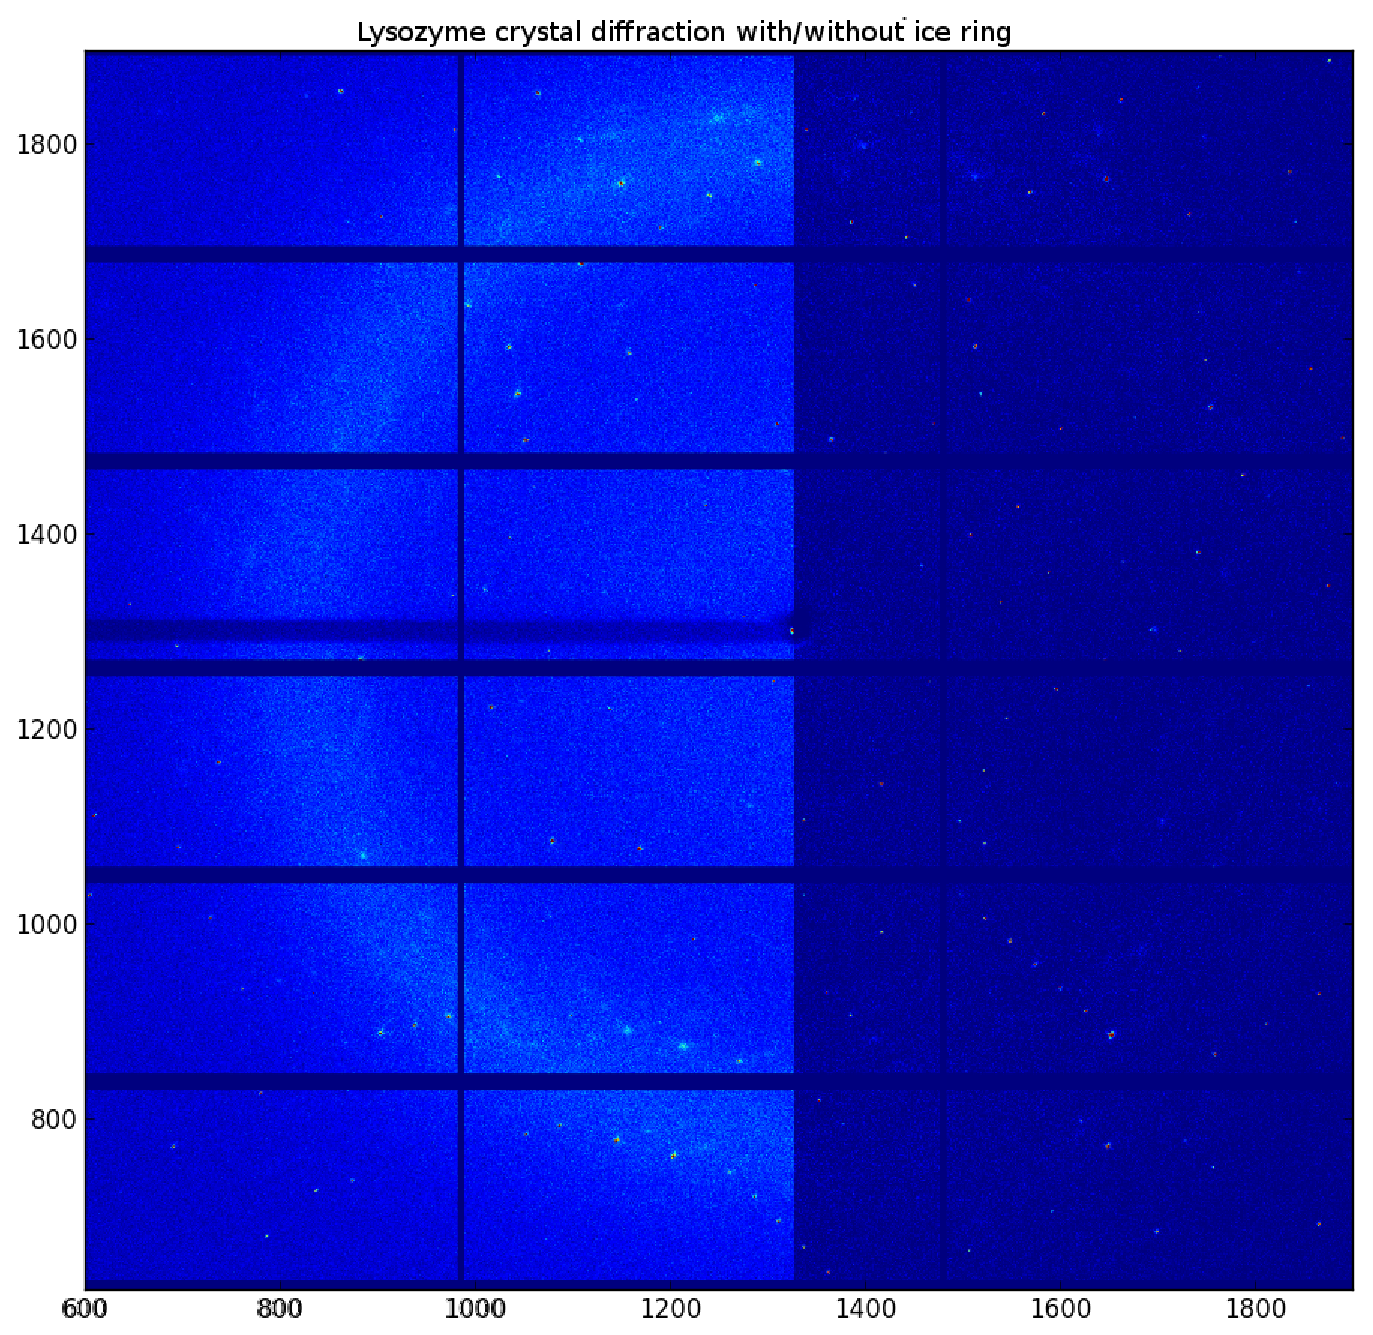
\includegraphics[width=15cm]{merged.eps}
\caption{Automatic removal of amorphous signal (ice ring) from Bragg peaks in a
protein crystallography experiment.}
\end{center}
\end{figure}

\subsubsection{Application to high-pressure diffraction}
When high-pressure diffraction is performed using diamond anvil cells, the Bragg
reflection from diamond tend to polluted the powder diffraction signal. PyFAI's
isotropic component separation can also be used to retrieve the pure powder
signal and discard the bragg diffraction signal from the the diamond.

\subsubsection{Application to serial crystallography}
In those experiment, tiny crystals in their medium (liquid) are sent in front of
the X-ray beam (using a jet or moving a motor) and data are acquired
continuously, using a fast detector (from dozens of Hertz to kHz).
Those experiment produce a huge amount of data and only a small fraction of the
frames contain actually diffraction signal.
PyFAI has been integrated into the processing software NanoPeakCell which
provides a graphical interface for frame selection in serial crystallography.
But pyFAI can also be integrated into the LImA data acquisition system
\cite{lima}, where it assesses the amount of single crystal
diffraction data within each frame and decide to save it or not.
By proceedings so, a huge amount of disk space and network bandwidth can be
saved.

\section{Conclusion}





\bibliographystyle{iucr}
\bibliography{biblio}
\appendix
\section{Project structure}
PyFAI is an open source project licensed under the GPL mainly written in Python (v2.6 or 2.7)
and heavily relying on the python scientific ecosystem: NumPy, SciPy and Matplotlib.
It provides high performances image treatment thanks to Cython and PyOpenCL.

The project is hosted on GitHub (https://github.com/kif/pyFAI) which provides
the issue tracker in addition to code hosting.
To ease the distribution, the
software is available as official Debian package and included in some of the
most famous Linux distribution like Ubuntu and Debian.
The program runs also on other operating systems like Windows and MacOSX.

Anybody can fork the project and adapt it to his own needs: CEA-saclay,
Synchrotrons Soleil and APS did it. If developments are useful to be shared,
they can be merged into the main branch via pull-requests.

\section{Parallel implementations using OpenCL}
Azimuthal integration and many other computing parts in pyFAI were written in
OpenCL kernels and interfaced using PyOpenCL \cite{pyopencl}. PyOpenCL offers a
shared execution model effective both on processors (CPU), graphics cars (GPU)
and accelerators like the Intel's Xeon Phi.

\subsection{Azimuthal Integration}
The direct azimuthal integration is basically a scatter operation which
requires large locked section.
To overcome this limitation, pixels have been
associated to the output bin of the histogram and stored in a look-up
table (LUT), making the integration look like a simple (if large and sparse)
matrix vector product.
The sparse matrix ``Compressed Sparse Row'' (CSR) format is now used in pyFAI,
saving about half of the space of the LUT previously used.
Secondly, all threads within a workgroup are collaborating to calculate the
matrix-vector product via a so-called ``parallel reduction'', offering
additional speed-up (especially on GPUs).
The compensated algebra (Kahan summation) is kept to maintain the precision
of the calculation while using single precision (32 bits) floating points
arithmetics. 

\subsection{Performances}
The table \ref{benchmark} shows the performance of pyFAI in frames processed per
second depending on the input image size (in semi-logarithmic scale). 
This
benchmark has been performed on a dual Intel Xeon E5-2667 (2.9Ghz) computer with a Nvidia Tesla K20 GPU and an Intel
Xeon Phi accelerator.

\begin{figure}
\label{benchmark}
\begin{center}
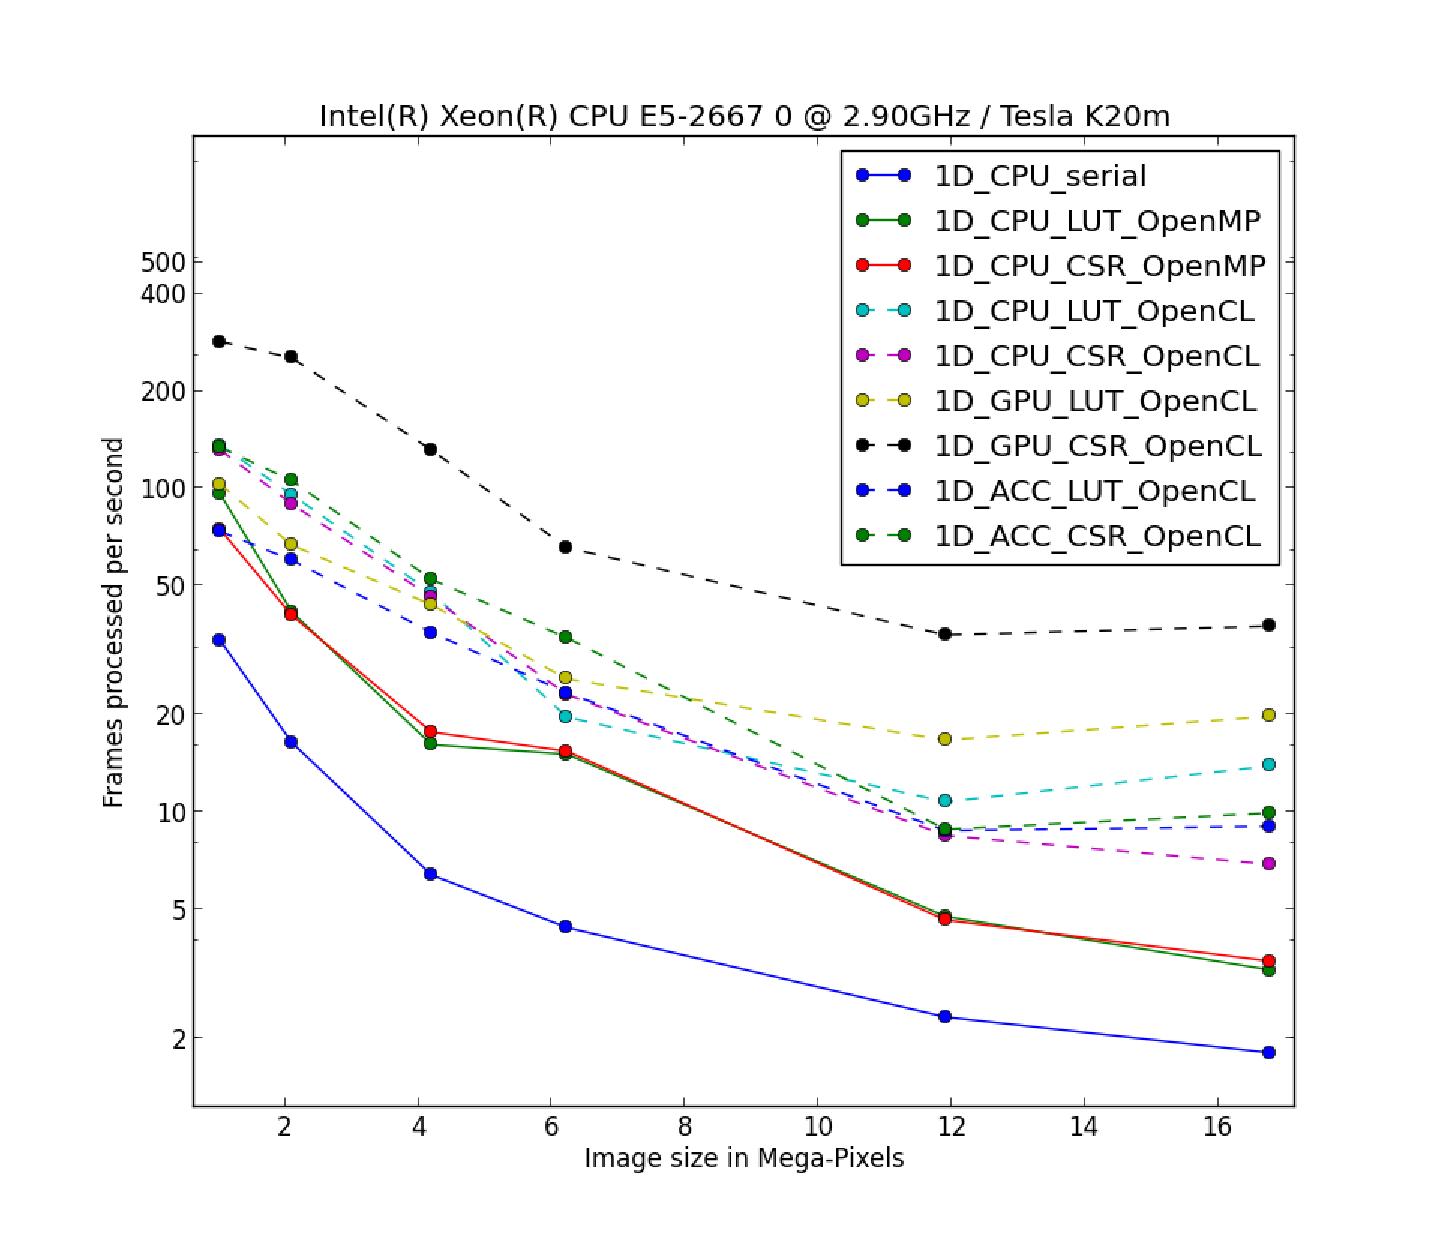
\includegraphics[width=5cm]{benchmark.eps}
\caption{Benchmark of the various algorithm to perform azimuthal integration in
pyFAI}
\end{center}
\end{figure}

In this benchmark, four group of curves can be extracted.
\begin{itemize}
  \item The lower plain blue curve presenting the serial Cython code using
  histograms (corresponding to the ``splitbbox'' method) which is the slowest
  implementation (even if it is 7x faster than a numpy implementation).
  \item The red and blue plain curves which correspond to the two parallel
  cython implementation for look-up tables.
  \item the group of dashed curves which represent the OpenCL optimized code
  running on the 12 CPU core, the 60 cores from the accerator or the GPU (LUT
  implementation).
  \item The upper curve, in dashed black correspond the CSR sparse matrix
  multiplication implemented in OpenCL code and running on the Tesla card which
  is twice faster
\end{itemize}  


\ack{Acknowledgements}

The author would like to thank all ESRF beamline teams for supporting the pyFAI
developement, especially BM01, ID02, ID11, ID13, BM26, ID29, BM29, ID30,
In the instrumentation division (ISDD) we would like to thank Claudio Ferrero,
head of data analysis unit, and Andy G\"otz, head of software group, for
supporting the algorithmic work performed on pyFAI in addition to the features
seen by the user.
V. Armando Solé, the author of PyMca, is also acknowledged for providing us some
important graphical user interface building blocks.  
The huge parallelization work on the core and porting to manycore devices
was mainly done by Dimitris Karkoulis, Zubair Nawaz and Giannis Ashiotis,
thanks the EU-grant LinkSCEEM-2 XXXX.

\end{document}
